\documentclass[12pt,a4paper]{article}
\usepackage[T2A]{fontenc}
\usepackage[utf8]{inputenc}
\usepackage[english,russian]{babel}
\usepackage[margin=22mm]{geometry}
\usepackage{amsmath,amssymb,booktabs,longtable,array}
\usepackage{graphicx}
\usepackage{float}
\usepackage{setspace}
\usepackage[hidelinks]{hyperref}
\setstretch{1.15}
\setlength{\parindent}{0pt}
\setlength{\parskip}{6pt}
\newcommand{\answer}[1]{\par\textbf{Как сказать на защите.} #1\par}
\newcommand{\warning}[1]{\par\textbf{Осторожно.} #1\par}
\begin{document}
\selectlanguage{russian}
\renewcommand{\contentsname}{Содержание}
\begin{center}
{\LARGE Как понять свою курсовую и подготовиться к защите}\[8pt]
{\large Анализ данных розничной торговли\\с помощью множественной регрессии}\[8pt]
Подробные пояснения для Максима Кибардина
\end{center}

Это учебный разбор вашей конкретной работы. Его задача --- объяснить каждое существенное решение: что сделали, зачем, что получилось и какое утверждение из этого действительно следует. Это не текст для чтения целиком во время выступления. Основная речь находится в \texttt{speech\_5min.md}; здесь разобраны также вопросы, которые могут задать после неё.

В пособие включены все семь рисунков из отчёта. Они расположены рядом с объяснениями: оси и обозначения, наблюдение на наших данных, допустимый вывод и короткий ответ на защите. Для сборки положите рядом с этим файлом каталог \texttt{figures/} с PNG; готовый комплект также сохранён в \texttt{defense\_guide\_bundle.zip}.

Сначала прочитайте разделы 1--5, затем разбор статистических проверок и результатов. В конце находятся готовые ответы и список распространённых ошибок. Формулы можно осваивать в два прохода: сначала смысл словами, потом обозначения. Матричные формулы нужны для понимания устройства расчёта; воспроизводить все их элементы наизусть обычно не требуется, если нет отдельного требования преподавателя.

Результаты соответствуют файлам \texttt{results/} и актуальному отчёту. Значения в тексте округлены. Предположения о происхождении исходных данных оговорены: описание источника не позволяет восстановить весь процесс построения агрегатов.

\tableofcontents
\clearpage
\section{Вся работа на одной странице}

\textbf{Что мы изучали?} Сумму продаж товара за месяц и её статистические связи с покупателями, конкурентными ценами и характеристиками товара.

\textbf{Какие данные?} 676 строк, 52 товара, 9 категорий, 20 месяцев: январь 2017 --- август 2018. Строка --- один товар в одном месяце. Это не 676 разных товаров и не 676 покупателей.

\textbf{Что сделали?} Проверили данные, изучили распределения и корреляции, построили несколько регрессий, оценили коэффициенты и их неопределённость, проверили остатки и чувствительность, сравнили предсказания на исключённых товарах.

\textbf{Основной вопрос.} Есть ли у конкурентных цен совместная связь с суммой продаж после учёта категории и других факторов?

\textbf{Ответ.} В основной расширенной модели совместный тест даёт $p=0{,}011$: на уровне 5\% гипотеза о трёх нулевых коэффициентах отвергается при принятой модели ошибок. После поправки Холма ни один конкурент индивидуально не выделяется. При добавлении календарных месяцев совместное p-value конкурентов возрастает до 0,061: статистическое решение чувствительно к учёту времени.

\textbf{Что ещё получилось?} Покупатели и вес значимы после поправки; вывод по весу пограничный ($p=0{,}049$). Добавление рейтинга, объёма и доставки повысило подгонку, но не улучшило ошибку предсказания на выбранном разбиении.

\textbf{Чего работа не устанавливает?} Причинного влияния, оптимальной цены, качества будущего прогноза или того, что все три конкурента обязательно важны по отдельности. Статистические проверки зависят от предположений об ошибках.

\answer{Я провёл последовательный анализ данных: от проверки смысла переменных до оценки качества модели на исключённых товарах. Главный результат --- в основной модели конкурентные цены дают совместный вклад, но при учёте календарных месяцев статистическое подтверждение ослабевает. Индивидуальное выделение конкретного конкурента после Холма неубедительно.}

\section{Что означает одна строка и почему это важно}

Представьте товар A в январе, тот же товар A в феврале и товар B в январе. Это три строки, но только два разных товара. У товара A в разных месяцах сохраняются многие свойства: вес, объём, фотографии и рейтинг. Продажи и конкурентное окружение могут меняться.

Такая таблица называется панельной: наблюдаем несколько объектов в разные моменты времени. Панель несбалансирована, потому что не каждый товар присутствует во всех 20 месяцах. Мы используем объединённую регрессию с категориями и кластерными ошибками, а не полноценную модель индивидуальных и временных фиксированных эффектов.

Повторные строки дают информацию о временных изменениях. Но для неизменного веса товара они не равны новым независимым измерениям веса разных товаров. Поэтому считать, что для всех выводов имеется 676 независимых объектов, неправильно.

\answer{Единица наблюдения --- товар--месяц. Одни и те же товары повторяются, поэтому я группировал стандартные ошибки по товару и при проверке предсказаний разделял целые товары.}

\section{Почему отклик --- сумма продаж, а не цена единицы}

В CSV есть три разных столбца:
\begin{itemize}
\item \texttt{unit\_price} --- цена единицы;
\item \texttt{qty} --- количество единиц;
\item \texttt{total\_price} --- выбранный денежный отклик.
\end{itemize}
Например, если одна единица стоит 50 и продано 10 единиц, денежная сумма равна 500. Рост суммы до 1000 мог возникнуть из-за роста количества до 20, а не из-за изменения цены единицы.

Мы проверили отношение
\[
 d_i=\frac{|T_i-U_iN_i|}{T_i}.
\]
Здесь $T_i$ --- \texttt{total\_price}, $U_i$ --- \texttt{unit\_price}, $N_i$ --- \texttt{qty}, $i$ --- номер строки, вертикальные черты означают модуль. Для 643 строк из 676 отличие меньше 0,3\%. Это поддерживает рабочую трактовку отклика как суммы продаж. Полной документации исходных транзакций нет, поэтому мы не выдаём эту трактовку за доказанное знание всех правил агрегирования. Валюта не установлена; доставка не прибавляется.

\textbf{Почему исключили цену единицы и количество?} Если одновременно объяснять сумму её почти точными множителями, получится преимущественно восстановление арифметической зависимости. Наш вопрос касается связей с конкурентным окружением и характеристиками товара. Сам факт высокой точности такой арифметической модели не сделал бы её ответом на этот вопрос.

\warning{Не говорите: «мы выяснили, как повысить цену». У нас другой отклик и нет причинного эксперимента. Не говорите также «эластичность спроса по цене»: для этого обычно изучают количество и собственную цену в специально обоснованной модели.}

\section{Зачем нужна множественная регрессия}

Парная связь сравнивает две переменные. Например, у более дорогих конкурентов может наблюдаться большая сумма продаж нашего товара. Но дорогие конкуренты могут чаще встречаться в другой категории, где продажи в целом выше. По одной корреляции эти объяснения не разделить.

Множественная регрессия описывает отклик через несколько факторов одновременно:
\[
 y_i=\beta_0+\beta_1x_{i1}+\cdots+\beta_kx_{ik}+\varepsilon_i.
\]
$y_i$ --- отклик; $x_{ij}$ --- фактор $j$ у строки $i$; $k$ --- число факторов без константы; $\beta_j$ --- коэффициент; $\beta_0$ --- свободный член; $\varepsilon_i$ --- часть отклика, не описанная уравнением.

«При прочих равных» означает, что включённые в уравнение остальные факторы мысленно фиксируются. Это свойство математического сравнения. Мы не проводили эксперимент и не подбирали реальные пары товаров, совпадающие буквально по всем свойствам. Неизвестные и пропущенные факторы всё ещё могут влиять на результат.

\answer{Множественная регрессия нужна, чтобы оценить связь каждого фактора при учёте остальных. Это позволяет отличать парную связь от условной и проверить совместный вклад блока конкурентных цен.}

\section{M1, M2, M3: как устроено сравнение}

Буква M означает модель; цифры --- условные номера спецификаций. Это не разные классы алгоритмов. Во всех случаях используем множественную линейную регрессию, изменяя набор объясняющих столбцов.

\begin{center}\small
\begin{tabular}{p{.10\textwidth}p{.61\textwidth}r}
\toprule Модель & Состав & Коэффициентов\\\midrule
M1 & Покупатели, три цены конкурентов, вес, фотографии & 7\\
M2 & M1 плюс восемь индикаторов категории & 15\\
M3 & M2 плюс рейтинг, логарифм объёма, доставка & 18\\
\bottomrule
\end{tabular}\end{center}

В M1 шесть числовых факторов и константа. В M3 девять числовых факторов, восемь категориальных индикаторов и константа. То есть 9 содержательных числовых характеристик плюс одна категориальная характеристика, которая записана восемью столбцами.

Сравнение M1 и M2 показывает, что меняется после учёта ассортимента. Сравнение M2 и M3 показывает роль трёх дополнительных характеристик. Все модели оценены на одних и тех же строках: изменение результата не вызвано подменой выборки.

В отчёте также есть S1--S3: каждая использует одного конкурента и одинаковые остальные факторы. Это вспомогательное сравнение. Они тоже являются множественными регрессиями: «один конкурент» не означает «только один признак».

\textbf{Почему M3 основная, если M2 предсказывает немного лучше?} M3 заранее выбрана для исследования расширенного набора связей. Способность предсказывать --- отдельный вопрос. Мы можем изучать коэффициенты полной модели и одновременно честно признать, что дополнительные факторы не помогли предсказанию. Это содержательный результат сравнения.

\section{Почему выбраны именно эти признаки}

\begin{longtable}{p{.24\textwidth}p{.31\textwidth}p{.37\textwidth}}
\toprule Признак & Зачем включён & Что важно помнить\\\midrule\endhead
Покупатели & Покупательская активность & Совпадает внутри категории и месяца; не подтверждённое число покупателей конкретного товара.\\
Цены трёх конкурентов & Основной вопрос конкурентного окружения & Механизм сопоставления конкурентов не документирован полностью.\\
Вес & Физическая характеристика & Постоянен внутри товара; связь оценивается между товарами.\\
Объём & Дополняет вес габаритами & Частично общая информация с весом; единица объёма не подтверждена.\\
Фотографии & Полнота карточки & Число фото не равно прямому измерению качества карточки.\\
Рейтинг & Оценка товара & Узкий диапазон; постоянен внутри товара; не доказанный причинный фактор.\\
Доставка & Условия продажи & В исходной шкале, ноль допустим; не включается в денежный отклик.\\
Категория & Различия ассортимента & Редкие категории представлены лишь двумя товарами.\\
\bottomrule
\end{longtable}

\textbf{Почему не все 30 столбцов?} Часть --- идентификаторы и календарь, часть почти восстанавливает отклик, смысл некоторых недостаточно ясен. Добавление множества похожих признаков увеличит неопределённость и затруднит объяснение. Мы сначала задаём вопрос, потом выбираем измеряющие его факторы.

\textbf{Почему оставили незначимые признаки?} Значимость --- результат исследования, а не обязательное условие включения. Если удалять все незначимые признаки после просмотра данных, изменяется смысл остальных коэффициентов и возникает дополнительный отбор, который тоже нужно учитывать. Полная и более простая модели позволяют показать, что дали дополнительные характеристики.

\textbf{Почему доставка допустима, хотя есть ноль?} Нельзя взять обычный логарифм нуля. Но доставку мы не логарифмируем: в исходной шкале ноль корректен. Сам по себе он не ошибка и не повод удалять строку.

\section{Как учитывается категория}

Нельзя заменить девять категорий числами от 1 до 9 и трактовать их как обычный числовой фактор: тогда возникнет искусственный порядок и равные расстояния между категориями.

Используются индикаторы. Например, $D_i=1$, если строка относится к определённой категории, и $D_i=0$ иначе. Для девяти категорий с константой нужно восемь индикаторов. Девятая становится базой.

Почему не девять? Сумма девяти индикаторов в каждой строке равна единице, то есть совпадает со столбцом константы. Возникает точная линейная зависимость. Исключение одного индикатора устраняет её.

База --- \texttt{garden\_tools}, одна из наиболее представленных категорий. Коэффициент другой категории описывает отличие среднего логарифма отклика от базы при фиксированных остальных факторах. Если поменять базу, коэффициенты категории и константа перепишутся, но предсказания той же модели сохранятся.

\warning{Категория --- контроль различий ассортимента, но не контроль всех свойств каждого товара. В работе нет индивидуального индикатора для каждого товара. В дополнительной проверке есть индикаторы календарных месяцев.}

\section{Что было сделано при очистке}

Проверены пропуски, дубликаты строк, повтор ключа «товар--месяц», типы, даты, допустимость значений, положительность логарифмируемых величин и конечность чисел. Проблем, требующих удаления, не найдено. Все 676 строк сохранены.

«Мы не удалили строки» не означает «очистка не проводилась». Корректный результат проверки может состоять в том, что данные допустимы. Нельзя удалять наблюдения только для демонстрации проделанной работы.

Большая сумма продаж может быть реальным наблюдением. Поэтому крайние значения не удаляются автоматически по статистическому порогу. Вместо этого далее проверяется, насколько меняется результат при исключении целого товара.

\answer{Я проверил качество данных и обосновал сохранение всех строк. Преобразовал даты, проверил ключ, ограничения логарифмов и почти арифметическую связь суммы с ценой и количеством.}

\section{Зачем логарифмировать}

Натуральный логарифм $\ln x$ переводит мультипликативные отношения в аддитивные. Например, $\ln(ab)=\ln a+\ln b$. Большие значения сжимаются: разница между 100 и 1000 превращается в разницу между примерно 4,605 и 6,908.

В исходной сумме продаж правый хвост длинный. Логарифм облегчает описание относительных изменений и уменьшает доминирование крупных абсолютных значений при подгонке. Но он не гарантирует правильную модель, нормальность ошибок или отсутствие выбросов.

Логарифмируются отклик, покупатели, три конкурентные цены, вес и объём. Рейтинг, фотографии и доставка входят в исходных единицах. Все логарифмируемые значения строго положительны.

\answer{Логарифмическая форма соответствует асимметрии данных и даёт относительную интерпретацию коэффициентов. Её пригодность я оценивал отдельно по диагностике и предсказаниям.}


\subsection{Как читать две гистограммы}

\begin{figure}[H]\centering
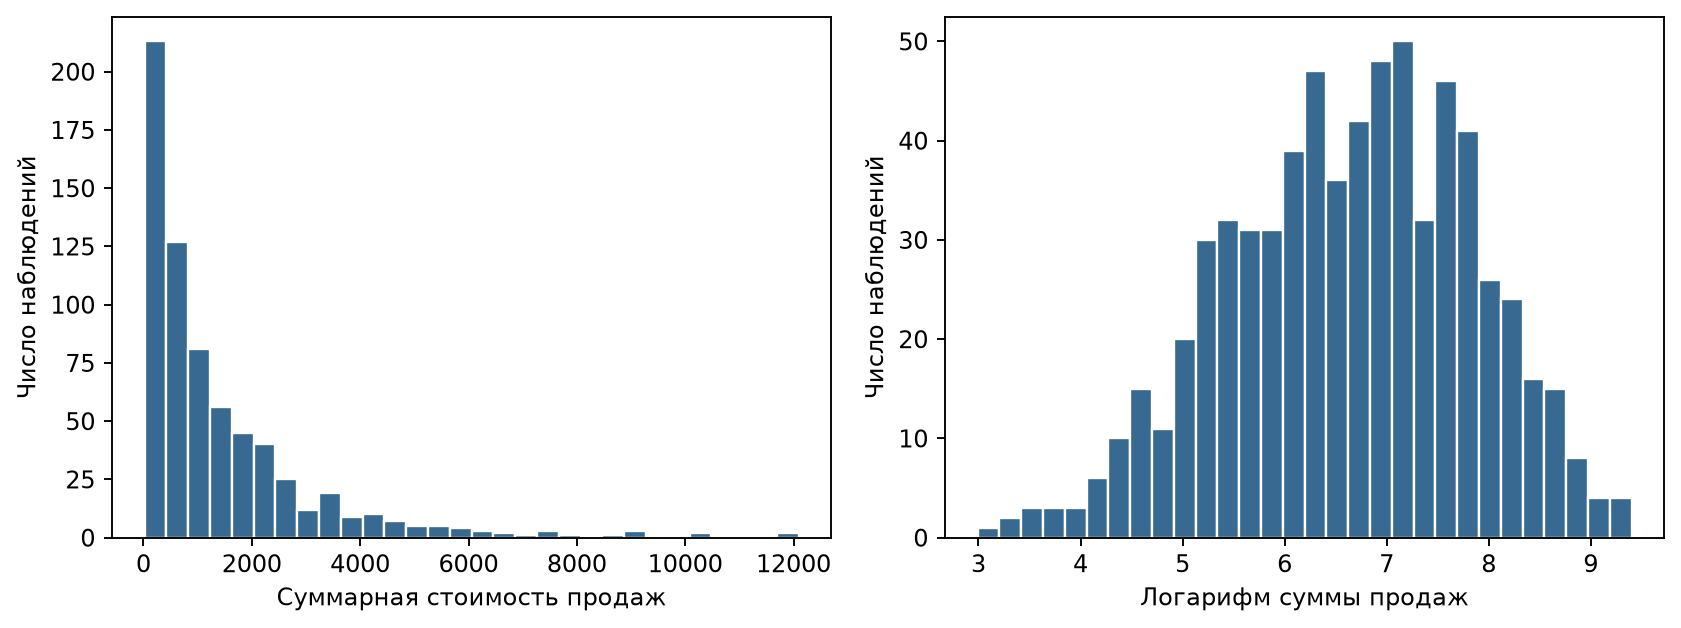
\includegraphics[width=0.98\textwidth,height=.48\textheight,keepaspectratio]{figures/distributions.png}
\caption{Одна сумма продаж на исходной и логарифмической шкалах}\label{learn:dist}
\end{figure}

\textbf{Что изображено.} Слева по горизонтали --- сумма продаж в исходных денежных единицах. Справа --- её натуральный логарифм. По вертикали на обеих панелях --- число строк, попавших в интервал значений. Это одни и те же 676 строк, показанные на разных шкалах.

\textbf{Как читать столбцы.} Высокий столбец означает, что в таком диапазоне много наблюдений. Он не показывает среднюю сумму и не является оценкой точности модели. Столбцы группируют соседние значения; ширина интервалов влияет на внешний вид гистограммы.

\textbf{Что видно у нас.} На исходной шкале основная масса наблюдений сосредоточена слева, а вправо тянется длинный хвост. Средняя сумма 1422,71 выше медианы 807,89. После логарифмирования большие значения сжимаются и расположение наблюдений становится удобнее для анализа. Значения справа на логарифмическом рисунке остаются большими суммами, просто на другой шкале.

\textbf{Что нам это дало.} Получили наглядное основание рассмотреть логарифмический отклик и относительные связи. Мы не удалили большие суммы и не заменили исходные данные вымышленными нормальными значениями.

\warning{Внешне более ровная гистограмма логарифма не доказывает нормальность ошибок, пригодность регрессии или причинность. Здесь показано распределение отклика, а не распределение остатков.}

\answer{Левая панель показывает асимметрию исходной суммы продаж. Правая показывает действие логарифма: он сжимает хвост и позволяет работать с относительными изменениями. Корректность модели я проверяю отдельно.}


\section{Что показывают корреляции}

Корреляция Пирсона описывает линейную парную связь на выбранных шкалах. Она лежит от $-1$ до $1$. Спирмен описывает связь рангов: важен порядок значений, а не только расстояния между ними. В нашей работе оба показателя используются описательно.

Корреляция покупателей с логарифмом суммы продаж около 0,432. У второго конкурента --- около 0,276. У объёма парная корреляция близка к нулю, но его коэффициент в полной модели положителен. Это возможно: после учёта категории и других факторов оценивается другая, условная связь.

Мы не считаем обычные p-value корреляций так, будто все строки независимы. Повторные наблюдения одного товара и общая активность категории делают такое упрощение сомнительным.

\warning{Корреляция не устанавливает причинность. Нулевая парная корреляция также не исключает нелинейной или условной связи.}


\subsection{Диаграммы рассеяния: что означает каждая точка}

\begin{figure}[H]\centering
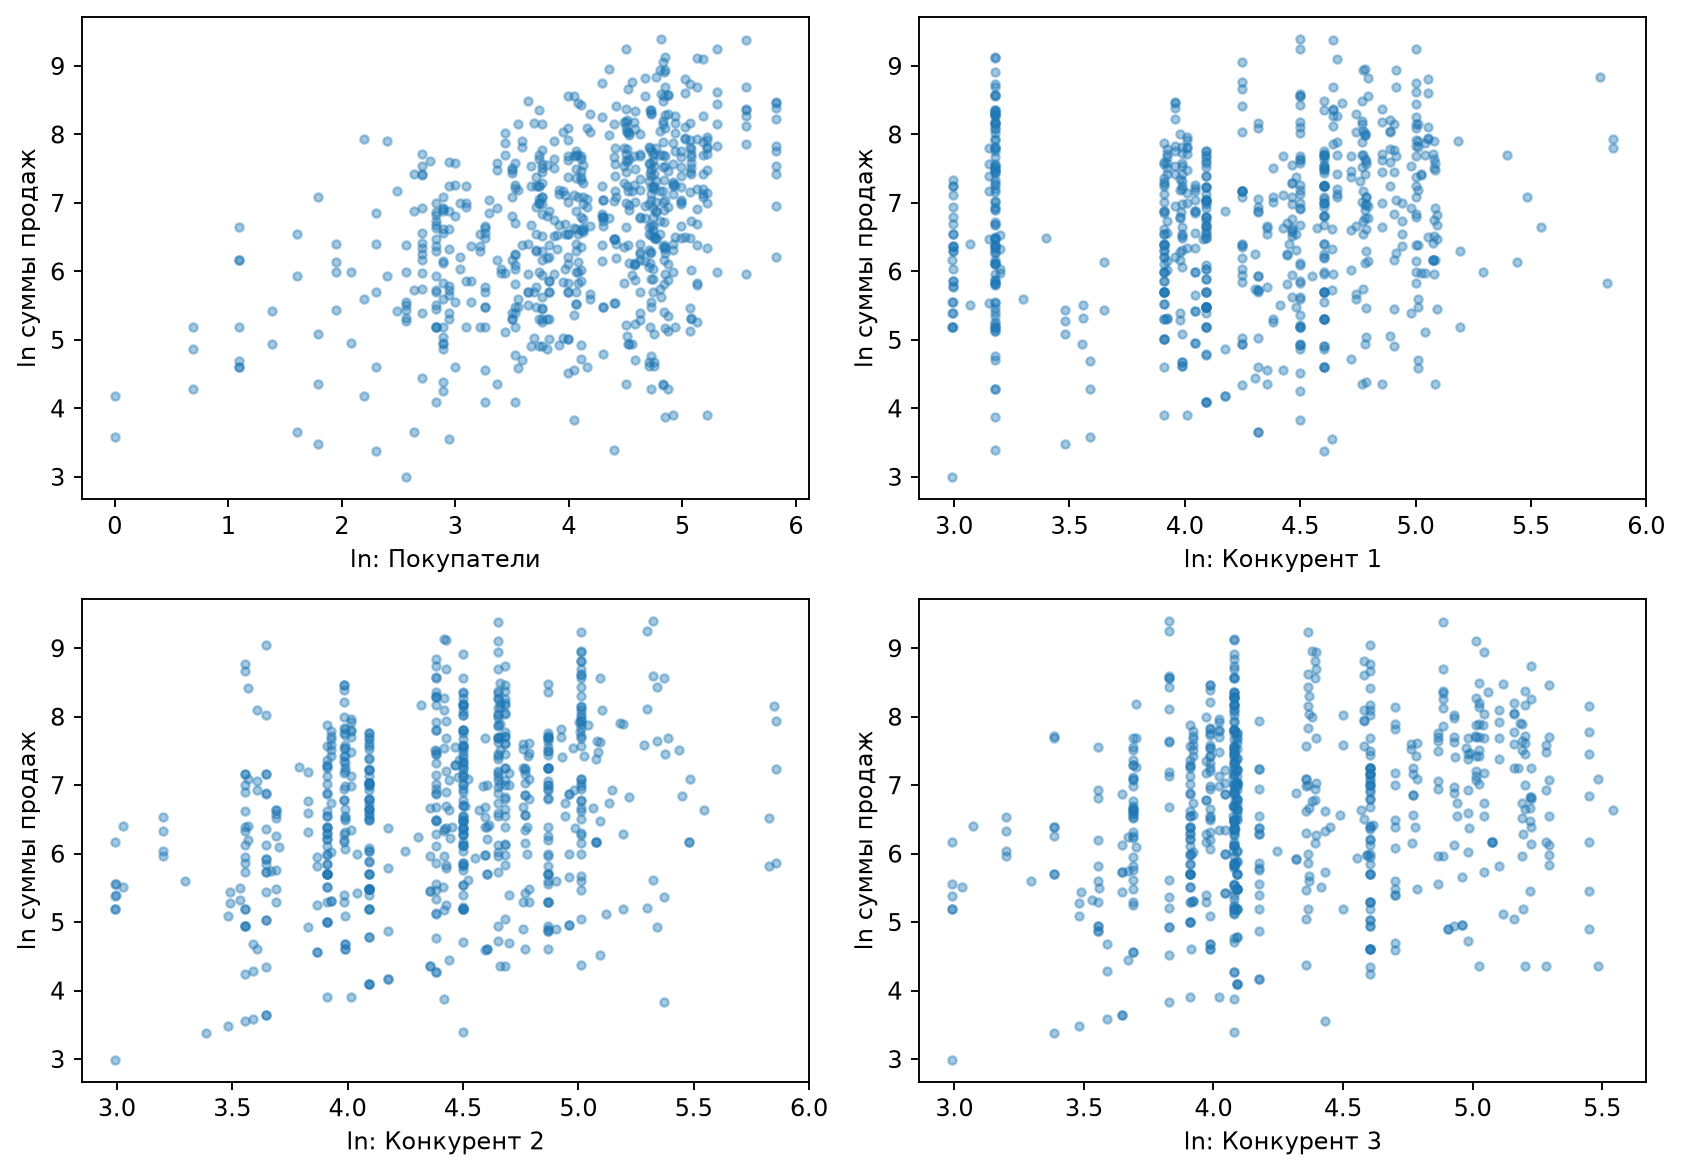
\includegraphics[width=0.98\textwidth,height=.57\textheight,keepaspectratio]{figures/relationships.png}
\caption{Парные связи покупателей и цен конкурентов с откликом}\label{learn:scatter}
\end{figure}

\textbf{Оси и точки.} Каждая точка --- строка «товар--месяц». По вертикали во всех четырёх панелях --- логарифм суммы продаж. По горизонтали --- логарифм покупателей (слева сверху) или одного из конкурентных ценовых показателей. Более высокая точка означает большую сумму продаж, более правая --- большее значение соответствующего фактора.

\textbf{Как выглядит связь.} Если облако в среднем поднимается слева направо, связь положительная. Если опускается --- отрицательная. Широкий разброс означает, что при похожем значении фактора наблюдаются разные суммы продаж. Точки могут накладываться, поэтому визуальное число точек не всегда равно числу строк.

\textbf{Что видно у нас.} У покупателей положительное направление заметнее, но разброс всё равно велик. Для конкурентных цен облака широкие; особенно нельзя по отдельным крайним точкам назвать точный коэффициент. Вертикальные полосы возникают из-за повторяющихся значений фактора. Они сами по себе не доказывают ошибку данных.

\textbf{Зачем это нужно.} Рисунок помогает увидеть форму парной связи, повторяющиеся значения и разброс до моделирования. Он объясняет, почему одного фактора недостаточно и зачем учитывать несколько факторов одновременно.

\warning{Это не графики коэффициентов M3: остальные факторы здесь не зафиксированы. На этих панелях нет линии регрессии, доверительного интервала или формальной проверки значимости.}

\answer{Каждая точка --- товар в месяце. Покупатели связаны с откликом положительно, но разброс большой. На следующем этапе я проверяю условные связи в множественной модели.}

\subsection{Тепловая карта: как читать цвета и числа}

\begin{figure}[H]\centering
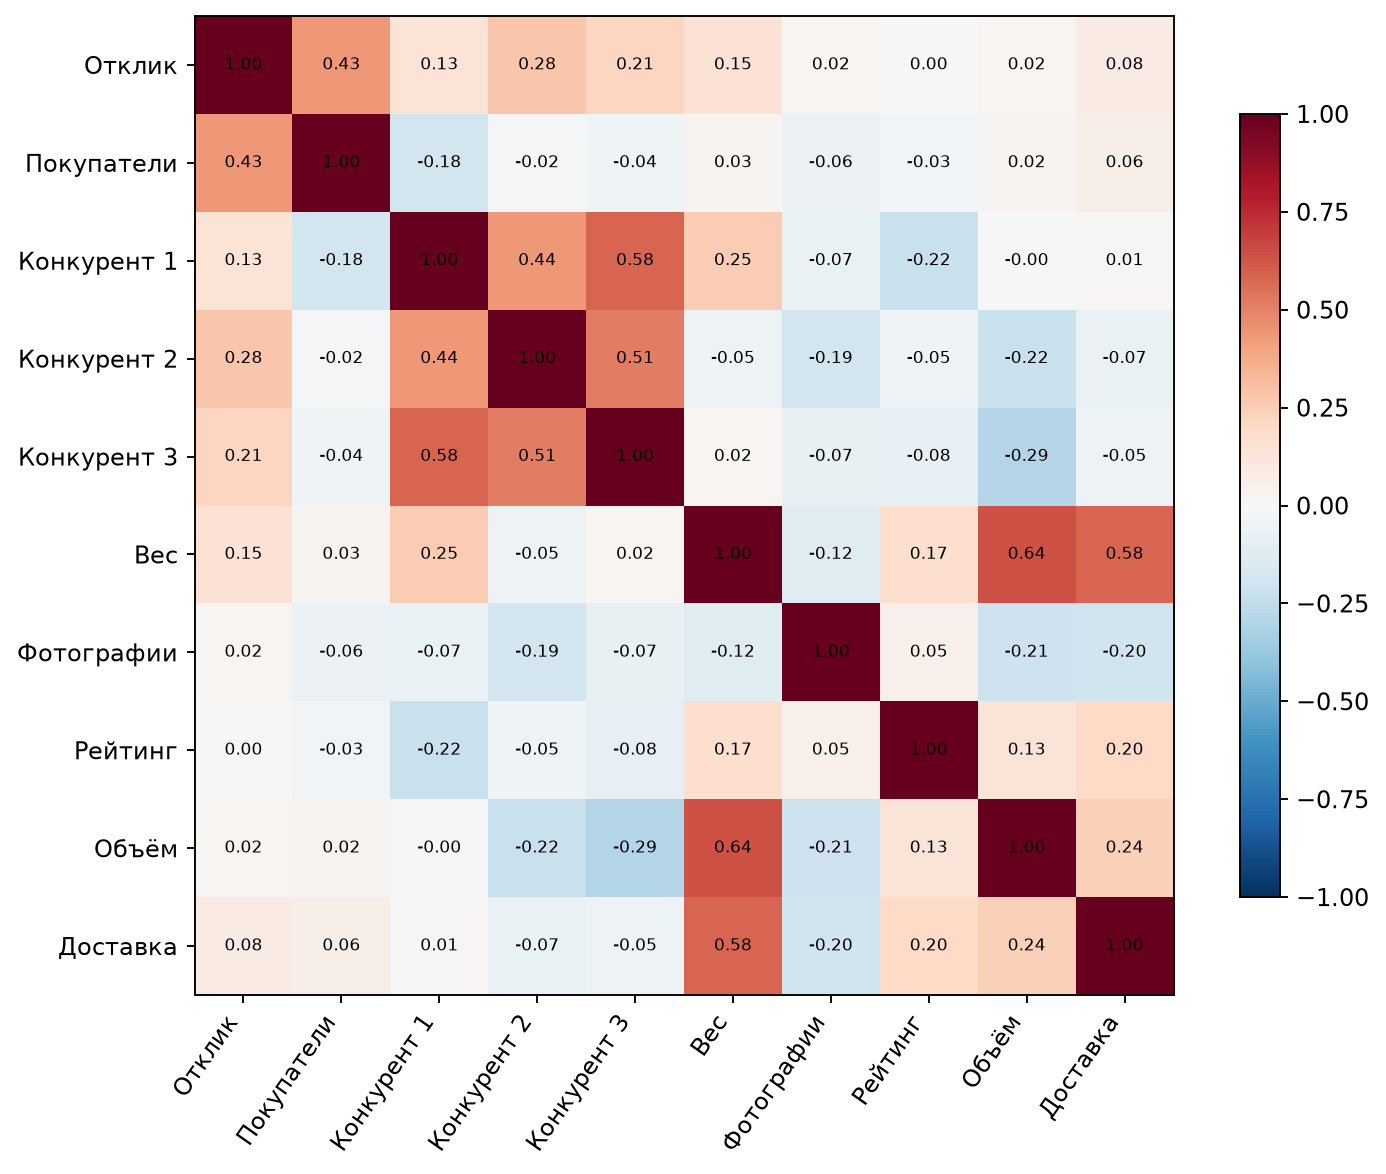
\includegraphics[width=0.98\textwidth,height=.62\textheight,keepaspectratio]{figures/correlations.png}
\caption{Корреляции на шкалах модели, без категориальных индикаторов}\label{learn:heatmap}
\end{figure}

\textbf{Как найти нужное число.} Выберите строку одного показателя и столбец другого; в пересечении стоит их корреляция Пирсона. Тёмно-красный цвет ближе к $+1$, тёмно-синий --- к $-1$, светлый --- к нулю. Диагональ всегда равна единице: переменная сравнивается сама с собой. Карта симметрична, поэтому читать обе её половины необязательно.

\textbf{Наши примеры.} Отклик и покупатели: около 0,43. Первый и третий конкуренты: около 0,58. Вес и объём: около 0,64. Последний пример показывает, почему габариты и масса могут нести частично общую информацию. Цвет у рейтинга и отклика почти белый: парная линейная связь близка к нулю.

\textbf{На каких шкалах это посчитано.} Отклик, покупатели, конкурентные цены, вес и объём логарифмированы. Фотографии, рейтинг и доставка --- в исходной шкале. Поэтому короткая подпись «Вес» на картинке обозначает здесь именно логарифм веса.

\textbf{Что нам это дало.} Получили предварительное описание парных связей и возможного дублирования. В полной модели это дополняется VIF, который учитывает сразу остальные числовые факторы и категориальные индикаторы. Индикаторов категории на самой карте нет.

\warning{Корреляция не является коэффициентом регрессии или p-value. Карта не доказывает независимость факторов. Небольшие парные корреляции не исключают линейного дублирования сразу несколькими столбцами; поэтому одной карты недостаточно.}

\answer{Карта показывает попарные связи. Например, вес и объём связаны, поэтому я проверил их совместное включение и чувствительность оценок. Это диагностика информации факторов, а не доказательство причинности.}

\subsection{Ящики с усами: зачем сравнивать категории}

\begin{figure}[H]\centering
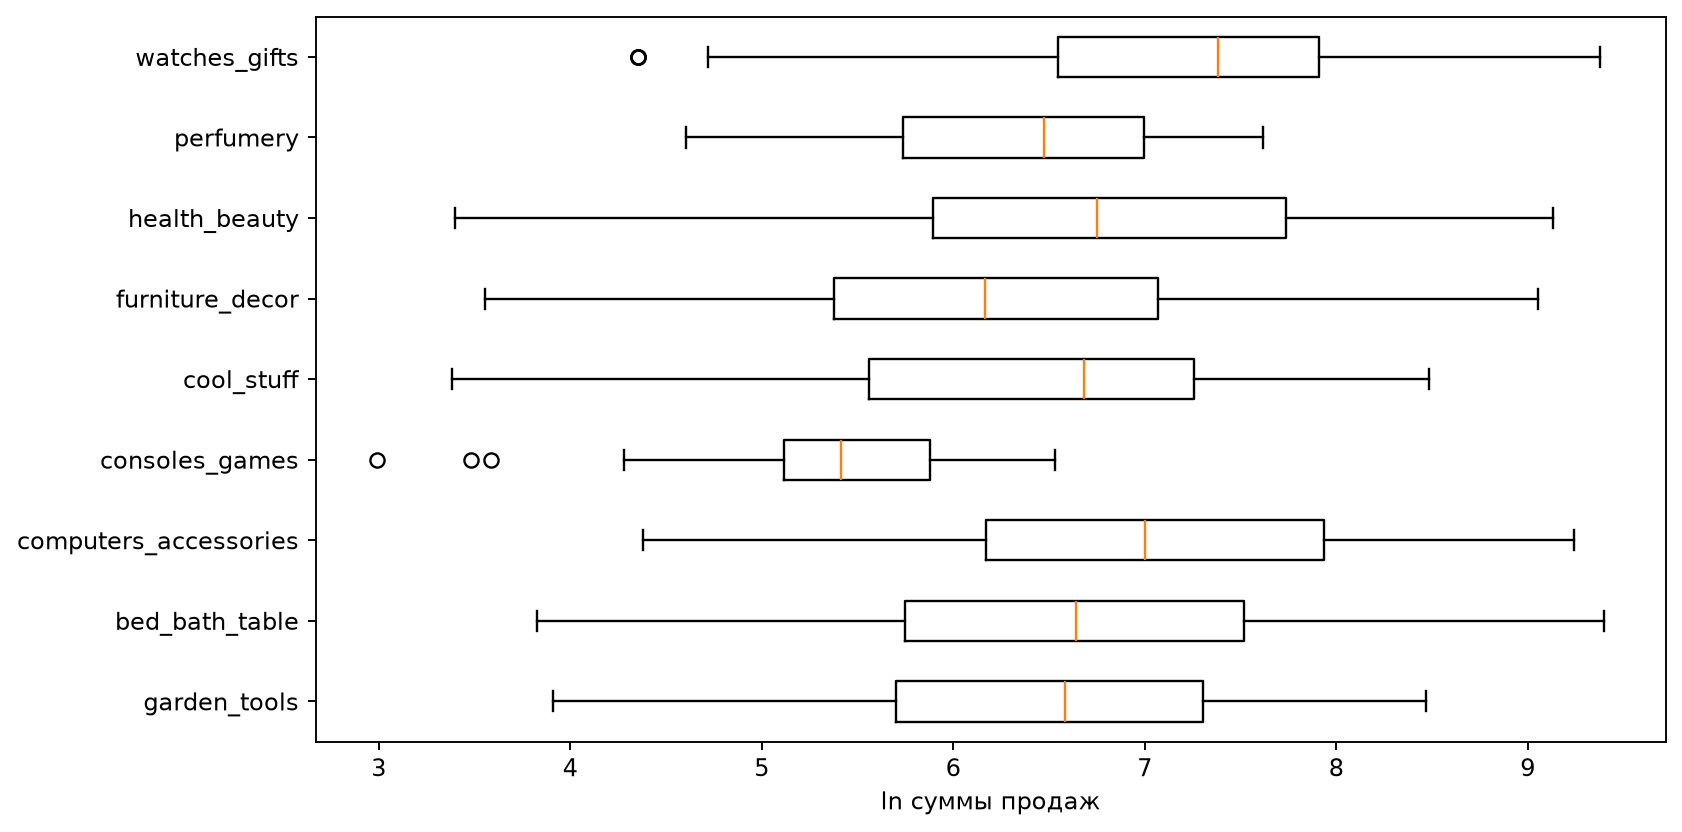
\includegraphics[width=0.98\textwidth,height=.53\textheight,keepaspectratio]{figures/categories.png}
\caption{Распределения логарифма суммы продаж по категориям}\label{learn:boxes}
\end{figure}

\textbf{Оси.} По вертикали перечислены категории, по горизонтали --- логарифм суммы продаж. У каждой категории свой горизонтальный ящик.

\textbf{Устройство ящика.} Оранжевая линия --- медиана, то есть середина упорядоченных значений. Левая и правая границы прямоугольника --- первый и третий квартили; между ними центральные 50\% строк. Длина ящика --- межквартильный размах. Усы доходят до крайних наблюдений в пределах стандартной границы 1,5 межквартильного размаха от квартилей. Отдельные кружки --- наблюдения за этими границами. Они не обязательно являются ошибками и из данных автоматически не удаляются.

\textbf{Что видно у нас.} Ящик \texttt{watches\_gifts} расположен правее, чем \texttt{consoles\_games}; типичные суммы различаются. При этом многие ящики и усы перекрываются: одна категория не определяет сумму однозначно. Усов и кружков недостаточно, чтобы судить о точности среднего или коэффициента категории.

\textbf{Что нам это дало.} Сравнение показывает, что ассортимент неоднороден. Это содержательная причина включить категорию в M2 и M3, а не считать все товары сопоставимыми только по конкурентной цене.

\warning{Границы ящика --- не доверительный интервал! График объединяет месячные строки, а не 676 независимых товаров. В двух категориях только по два разных товара. Различия на рисунке ещё не очищены от остальных факторов.}

\answer{Ящик показывает медиану и разброс логарифма суммы продаж внутри категории. Различия категорий мотивируют контроль ассортимента, но график сам по себе не проверяет условные коэффициенты и не доказывает причинное влияние категории.}


\section{МНК: откуда берутся коэффициенты}

Модель даёт расчётное значение $\widehat y_i$. Шляпка означает, что величина оценена по данным. Остаток
\[
 e_i=y_i-\widehat y_i
\]
равен наблюдаемому минус предсказанное. Если он положительный, модель недооценила отклик, если отрицательный --- переоценила.

Метод наименьших квадратов выбирает коэффициенты, минимизирующие
\[
 \sum_{i=1}^{n}e_i^2.
\]
$\sum$ означает сумму по всем $n=676$ строкам. Квадраты не дают положительным и отрицательным остаткам погасить друг друга и сильнее штрафуют крупные отклонения. Мы минимизируем ошибки логарифма, поэтому это не то же самое, что минимизировать денежные ошибки исходных сумм.

В матричной форме
\[
 \widehat{\boldsymbol\beta}=(X^\top X)^{-1}X^\top y.
\]
$X$ --- таблица модельных столбцов с константой, $y$ --- столбец логарифмов суммы продаж, $\boldsymbol\beta$ --- вектор коэффициентов, $\top$ --- транспонирование, $^{-1}$ --- обратная матрица. Формула требует полного ранга: один столбец не должен точно выражаться через другие. В коде используется \texttt{statsmodels.OLS.fit}; коэффициенты независимо проверены через \texttt{numpy.linalg.lstsq}.

\section{Что означают коэффициент, ошибка и стандартная ошибка}

Нужно различать три понятия.
\begin{enumerate}
\item \textbf{Коэффициент} --- направление и величина модельной связи. Например, коэффициент логарифма покупателей $0{,}686$.
\item \textbf{Остаток} --- ошибка предсказания отдельной строки на обучении: $e_i=y_i-\widehat y_i$.
\item \textbf{Стандартная ошибка коэффициента} --- оценка неопределённости самого коэффициента при изменении выборки. У покупателей она около $0{,}0669$.
\end{enumerate}

Не бывает вывода «стандартная ошибка покупателей равна 0,067 покупателя»: это ошибка коэффициента, а не измерения числа людей. Также её нельзя путать со стандартным отклонением остатков.

\subsection{Что такое SEcluster}

SE означает standard error, стандартная ошибка. Индекс cluster означает, что расчёт учитывает группировку строк. У одного товара месячные ошибки могут быть связаны: неизвестная популярность товара влияет сразу на несколько месяцев. Если объявить эти строки независимыми, точность коэффициента можно переоценить.

Кластерная оценка допускает зависимость и неодинаковую дисперсию внутри товара. Используется CR1 с поправкой для конечной выборки. Число групп $G=52$. Матрица ковариаций коэффициентов обозначается $\widehat{\mathcal V}$, а
\[
 \operatorname{SE}_{cluster}(\widehat\beta_j)=\sqrt{\widehat{\mathcal V}_{jj}}.
\]
Индекс $jj$ означает диагональный элемент для коэффициента $j$. Ковариации вне диагонали нужны, когда проверяем несколько коэффициентов совместно.

\textbf{Что меняется от кластеризации?} Коэффициенты того же МНК остаются прежними; меняются оценка их неопределённости, p-value и интервалы. Мы не «улучшаем предсказание кластеризацией».

\textbf{Главная оговорка.} Разные товарные группы предполагаются независимыми по ошибкам. Общие шоки категории или месяца могут затрагивать несколько товаров. Кластеризация только по товару этого полностью не покрывает. Само совпадение регрессора у товаров ещё не доказывает корреляцию ошибок, но указывает на возможный общий уровень воздействия. Поэтому точность статистических выводов ограничена.

\section{Гипотезы, t-статистика и p-value}

\subsection{Почему выбраны именно эти проверки}

Здесь выбор делается по проверяемому вопросу, а не по принципу «какой критерий даст маленькое p-value».
\begin{itemize}
\item \textbf{Один коэффициент: t-проверка.} У нас уже есть оценённая регрессия. Вопрос: отличается ли её коэффициент от нуля при учёте остальных факторов? Оценка, делённая на её стандартную ошибку, --- естественная статистика для одного такого ограничения. Это t-проверка коэффициента регрессии, а не сравнение средних двух произвольно выделенных групп.
\item \textbf{Несколько коэффициентов: совместный Вальд в F-форме.} Вопрос о трёх конкурентах относится сразу к трём ограничениям. По отдельным p-value ответить на него нельзя: совместная проверка учитывает также ковариации оценок. Используем ту же кластерную ковариацию, что и для t-проверок.
\item \textbf{Повторные товары: кластерные ошибки.} Месячные строки одного товара могут иметь общие ненаблюдаемые причины отклонений. Обычный расчёт для независимых строк этого не учитывает. Кластеризация выбрана по устройству данных; она не требует сначала получить значимый тест ненормальности или неодинаковой дисперсии.
\item \textbf{Неопределённость величины: доверительный интервал.} Одного слова «значимо» недостаточно. Интервал показывает, насколько широкий диапазон коэффициента совместим с оценкой в используемой процедуре. Это интервал коэффициента, а не прогнозный интервал продаж отдельного товара.
\item \textbf{Девять индивидуальных вопросов: Холм.} Требуется контролировать риск хотя бы одного ложного отклонения внутри выбранного семейства. Метод Холма рассчитан именно на такой контроль и не требует независимости девяти проверок, если исходные p-value корректны.
\end{itemize}

\warning{Это обоснование применимости выбранного подхода при предпосылках, а не доказательство их выполнения. t- и F-распределения при кластеризации являются приближениями. Ненормальность исходного признака не запрещает МНК; общие ошибки разных товаров могут ограничить точность нашего вывода. Мы не выдаём наличие 52 товарных групп за автоматическое доказательство надёжности каждого теста.}

\answer{Для отдельного регрессионного коэффициента я использую t-проверку, для нескольких линейных ограничений --- совместный критерий Вальда. Ошибки кластеризованы по товару из-за повторных месяцев. Интервалы показывают неопределённость величины связи, а поправка Холма учитывает девять индивидуальных проверок. Все выводы условны на принятой модели ошибок.}


Для отдельного коэффициента проверяем
\[
 H_0:\beta_j=0,\qquad H_1:\beta_j\ne0.
\]
$H_0$ --- нулевая гипотеза об отсутствии линейного вклада данного фактора при включённых остальных факторах; $H_1$ --- двусторонняя альтернатива.

\[
 t_j=\frac{\widehat\beta_j}{\operatorname{SE}_{cluster}(\widehat\beta_j)}.
\]
Статистика показывает, на сколько стандартных ошибок оценка отстоит от нуля. Для покупателей $0{,}6864/0{,}06685\approx10{,}27$. Для доставки оценка почти нулевая относительно её ошибки, поэтому $t$ близка к нулю.

\textbf{Что такое p-value?} Если предположить, что $H_0$ верна и используемая модель ошибок подходит, насколько необычна статистика такой же или большей экстремальности? Малое значение говорит против $H_0$ в этой модели.

Для двустороннего теста
\[
 p_j=2\{1-F_{t_{51}}(|t_j|)\}.
\]
$F_{t_{51}}(u)$ --- вероятность значения не больше $u$ в распределении Стьюдента с 51 степенью свободы; $|t_j|$ --- модуль; множитель 2 учитывает обе стороны отклонения от нуля.

Почему 51, а не 675 или 658? Это выбранное приближение для кластерного вывода: $G-1=52-1$. Для остаточных степеней свободы МНК используется другая величина $n-p=676-18=658$, где $p$ здесь число коэффициентов. Она участвует в других формулах. Не смешивайте два расчёта.

Порог $\alpha=0{,}05$ выбран как правило принятия решения. Если p-value меньше порога, $H_0$ отвергается. Сторона гипотезы выбрана двусторонней: ожидаемый положительный знак не является разрешением игнорировать отрицательные результаты.

\warning{p-value не означает вероятность, что гипотеза верна, вероятность случайности результата или величину эффекта. При $p=0{,}151$ нельзя сказать «вероятность отсутствия связи 15,1\%».}

\section{Доверительный интервал: смысл и вычисление}

Интервал отдельного коэффициента:
\[
 \widehat\beta_j\pm t_{0{,}975;51}\operatorname{SE}_{cluster}(\widehat\beta_j).
\]
Знак $\pm$ означает две границы: вычесть и прибавить. $t_{0{,}975;51}\approx2{,}008$ --- квантиль, слева от которого 97,5\% вероятности. По 2,5\% остаётся в каждом хвосте.

Для покупателей интервал примерно $[0{,}552;0{,}821]$. Он показывает неопределённость оценки коэффициента. Для второго конкурента интервал $[-0{,}303;0{,}807]$: с используемой точностью модель допускает и отрицательные, и положительные значения.

Смысл уровня 95\% относится к процедуре: в повторных выборках при подходящих предпосылках примерно 95\% таких интервалов накрывали бы истинный фиксированный коэффициент. Это не интервал, в котором лежат 95\% строк или 95\% индивидуальных продаж.

При одной двусторонней проверке на 5\% интервал исключает ноль тогда, когда соответствующий нескорректированный тест отвергает ноль. После поправки Холма решение может измениться, потому что она решает другую задачу контроля ошибки по нескольким тестам.

\section{Почему нужна поправка Холма}

Если много раз искать значимость на уровне 5\%, возрастает риск хотя бы одного ложного обнаружения. Наше семейство --- девять индивидуальных коэффициентов числовых факторов M3. Оно не включает все исследовательские проверки работы.

Холм сортирует p-value и сравнивает самые маленькие с более строгими порогами. Он контролирует вероятность хотя бы одного ложного отклонения в семействе при корректных исходных p-value. В коде используется \texttt{multipletests(method='holm')}.

Показательный пример --- вес. Исходное $p\approx0{,}00613$; это второе по малости p-value из девяти. На этом шаге множитель равен 8: $8\cdot0{,}00613\approx0{,}0490$. После учёта порядка шагов итоговое значение равно 0,0490. Вывод остаётся значимым, но близок к 0,05.

Для объёма исходное $p\approx0{,}0286$, после Холма около 0,200. Для третьего конкурента исходное 0,0352, после Холма около 0,211. Индивидуальные интервалы этих коэффициентов исключают ноль, но семейная проверка уже не выделяет их.

\answer{В таблице интервалы индивидуальные, а p-value Холма учитывают девять проверок. Поэтому интервал может исключать ноль, хотя решение после поправки незначимо. Это разные уровни контроля ошибки.}

\warning{Поправка не устраняет неудачную модель ошибок, не доказывает причинность и не учитывает автоматически весь предыдущий поиск моделей на этих данных.}

\section{Совместный F-критерий Вальда}

Главная гипотеза: все три коэффициента конкурентных цен одновременно равны нулю. Это другой вопрос, чем «каждый из них по отдельности значим».

Совместный тест использует оценки и их ковариации. Если два фактора несут частично общую информацию, вклад блока может быть заметен, а разделить вклад между его столбцами трудно. Кроме того, индивидуальные проверки у нас строже из-за Холма. Это делает совместную значимость без индивидуального выделения вполне возможной; сам VIF не доказывает конкретное объяснение результата.

Формально ограничения записываются $A\boldsymbol\beta=c$, и
\[
 F_W=\frac1q(A\widehat{\boldsymbol\beta}-c)^\top
 (A\widehat{\mathcal V}A^\top)^{-1}(A\widehat{\boldsymbol\beta}-c).
\]
$A$ выбирает проверяемые коэффициенты; $c$ задаёт значения при $H_0$ (у нас нули); $q$ --- число ограничений; $\widehat{\mathcal V}$ --- кластерная ковариационная матрица; $\top$ --- транспонирование; $^{-1}$ --- обращение матрицы. Для конкурентов $q=3$. Используется F-приближение с 3 и 51 степенями свободы.

Это не обычный F-тест сравнения сумм квадратов при независимых ошибках. В коде \texttt{f\_test} вызван для результата с кластерной ковариацией.

\begin{center}\small
\begin{tabular}{lrr}
\toprule Проверка M3 & F & p-value\\\midrule
Три конкурентные цены & 4,100 & 0,011\\
Рейтинг, объём, доставка & 1,843 & 0,151\\
Восемь категориальных коэффициентов & 7,007 & $<0{,}001$\\
Все 17 коэффициентов без константы & 20,534 & $<0{,}001$\\
\bottomrule\end{tabular}\end{center}

Совместная связь конкурентов сохраняется и до расширения: M1 даёт $p<0{,}001$, M2 --- $p=0{,}018$. Это сопоставление спецификаций на одном наборе, а не три независимых эксперимента. Оно относится к моделям без календарного контроля; дополнительная проверка времени меняет решение на уровне 5\%.

\answer{Я отвергаю гипотезу, что все три коэффициента одновременно нулевые, при принятой модели ошибок. Это не доказывает значимость каждого и не позволяет назвать одного конкретного конкурента главным.}

\section{Как читать таблицу результатов M3}

Каждая строка --- коэффициент определённого фактора при учёте остальных. Столбцы: оценка, её кластерная стандартная ошибка, исходное p-value, p-value после Холма и индивидуальный интервал.

\begin{center}\small\begin{tabular}{lrrrrr}
\toprule
Фактор & $\widehat\beta$ & SE & $p$ & $p_{Holm}$ & 95\%-ный ДИ \\
\midrule
Покупатели & 0,686 & 0,067 & $<0{,}001$ & $<0{,}001$ & [0,552; 0,821] \\
Конкурент 1 & 0,195 & 0,144 & 0,182 & 0,728 & [-0,094; 0,484] \\
Конкурент 2 & 0,252 & 0,277 & 0,367 & 1,000 & [-0,303; 0,807] \\
Конкурент 3 & 0,447 & 0,207 & 0,035 & 0,211 & [0,032; 0,862] \\
Вес & 0,314 & 0,110 & 0,006 & 0,049 & [0,094; 0,535] \\
Фотографии & 0,126 & 0,060 & 0,041 & 0,211 & [0,006; 0,246] \\
Рейтинг & -0,029 & 0,305 & 0,925 & 1,000 & [-0,642; 0,584] \\
Объём & 0,335 & 0,149 & 0,029 & 0,200 & [0,036; 0,634] \\
Доставка & $0{,}000105$ & 0,011 & 0,993 & 1,000 & [-0,022; 0,022] \\
\bottomrule
\end{tabular}\end{center}

\textbf{Покупатели.} Положительный коэффициент 0,686, малая ошибка, очень маленькое p-value даже после поправки. Связь заметна в выбранной спецификации и знак устойчив к исключениям товара. Нельзя утверждать, что увеличение числа покупателей экспериментально вызовет именно такую прибавку: активность категории и продажи могут быть совместно определены.

\textbf{Вес.} Положительная оценка 0,314; после Холма p-value 0,049. Формальное правило на уровне 5\% даёт значимость, но вывод пограничный. Не следует называть его безусловно надёжным или универсальным.

\textbf{Конкуренты.} У всех точечные оценки положительные. Но после Холма ни один не выделяется индивидуально. У третьего исходное p-value меньше 0,05; это ещё не результат после поправки. Положительный знак не равен доказанной связи.

\textbf{Объём и фотографии.} Исходные p-value меньше 0,05, после Холма --- больше. Это исследовательские признаки с положительными оценками, но индивидуальные выводы по выбранному семейному правилу не подтверждены.

\textbf{Рейтинг и доставка.} Оценки близки к нулю относительно их ошибок; при исключении товаров даже знак меняется. Правильный вывод --- недостаточно информации для уверенной связи в этой модели. Неправильный --- «рейтинг и доставка вообще не имеют значения».

\section{Как получить проценты из коэффициента}

Если логарифмированы и отклик, и фактор, коэффициент приблизительно показывает процентную связь при росте фактора на 1\%. Для роста на 10\% лучше использовать точное выражение:
\[
 \Delta=100\{1{,}1^b-1\}\%.
\]
$b$ --- коэффициент нужного логарифмированного фактора; $1{,}1$ --- отношение нового значения фактора к старому. Для покупателей $b=0{,}6864$:
\[
 100(1{,}1^{0{,}6864}-1)\approx6{,}76\%.
\]
Умножение $0{,}6864\cdot10\%=6{,}864\%$ является приближением; в отчёте используется точная формула. Для веса результат около 3,04\%.

Если фактор входит в исходной шкале, при увеличении на $h$ единиц:
\[
 \Delta=100\{e^{bh}-1\}\%.
\]
$e^{bh}=\exp(bh)$ --- экспонента. Для фотографии $h=1$; оценка 0,126 даёт около 13,43\%. Для рейтинга выбран понятный шаг 0,1 балла. Для доставки шаг --- одна денежная единица исходного показателя. Большая точечная оценка фотографий не отменяет отсутствия индивидуального подтверждения после Холма.


\subsection{Точки с горизонтальными интервалами: как читать эффекты}

\begin{figure}[H]\centering
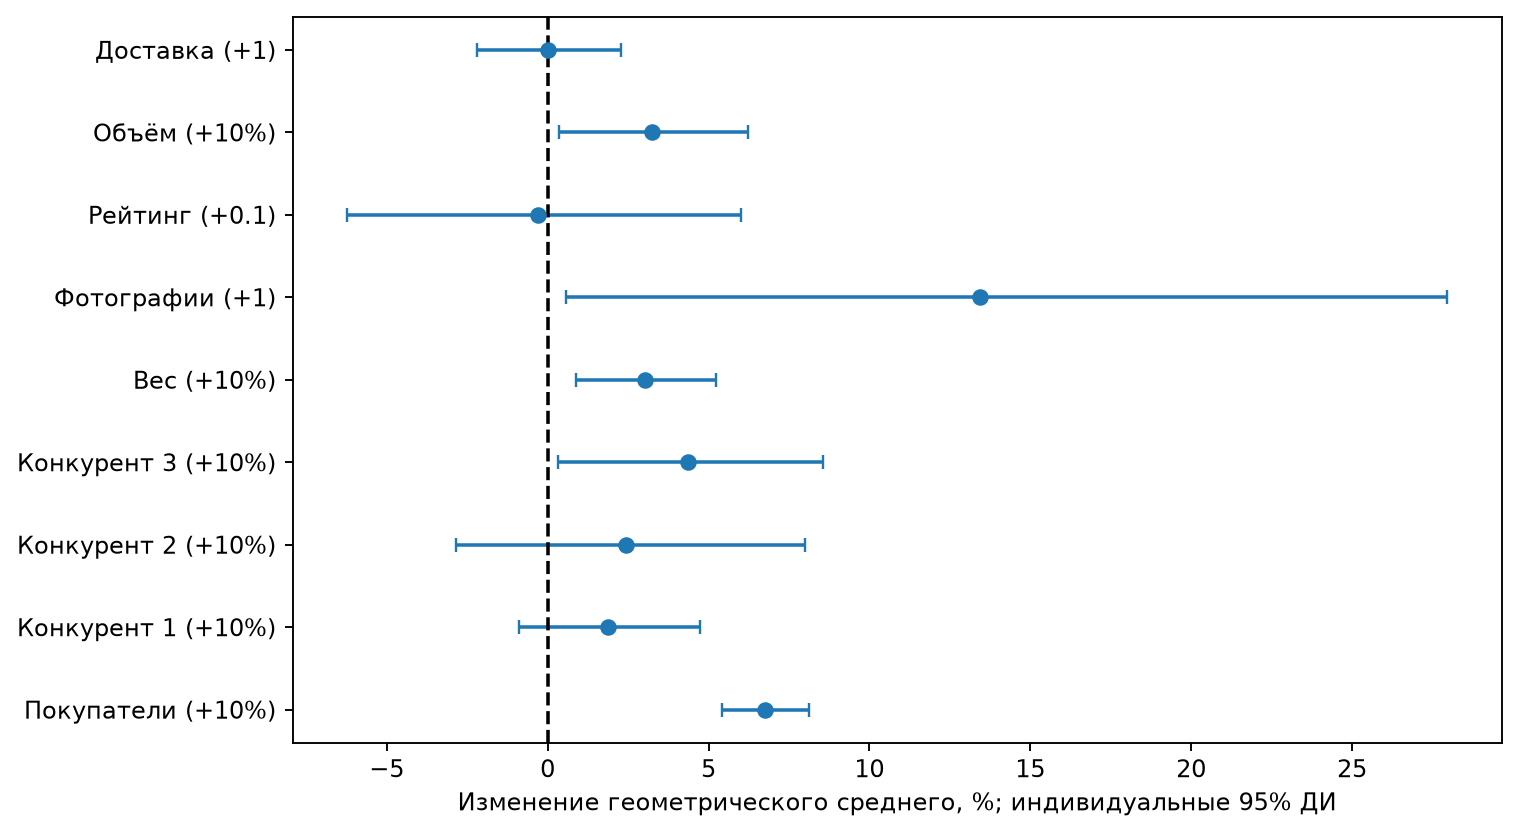
\includegraphics[width=0.98\textwidth,height=.53\textheight,keepaspectratio]{figures/effects.png}
\caption{Относительные связи M3 с индивидуальными 95\%-ными интервалами}\label{learn:effects}
\end{figure}

\textbf{Оси.} Строка соответствует фактору. В подписи указан шаг: для логарифмированных факторов $+10\%$, для фотографий $+1$, для рейтинга $+0{,}1$, для доставки $+1$ исходная денежная единица. По горизонтали --- модельная процентная связь с геометрическим средним суммы продаж.

\textbf{Что означает точка.} Это преобразованная оценка коэффициента, а не отдельный товар. Например, точка покупателей расположена около $+6{,}76\%$: это результат формулы с ростом фактора на 10\%.

\textbf{Что означает отрезок.} Это индивидуальный 95\%-ный интервал, полученный из кластерного интервала коэффициента. Чёрная вертикальная пунктирная линия --- ноль, то есть отсутствие изменения в такой интерпретации. Если отрезок пересекает ноль, нескорректированная двусторонняя проверка не отвергает нулевой коэффициент на уровне 5\%. Чем длиннее отрезок, тем больше неопределённость на выбранной шкале шага.

\textbf{Что видно у нас.} Покупатели дают положительную оценку и интервал примерно $[5{,}40;8{,}14]\%$. Первый и второй конкуренты имеют интервалы, пересекающие ноль. У третьего конкурента, объёма и фотографий индивидуальные интервалы ноль исключают, но после Холма их коэффициенты не выделяются. У рейтинга и доставки оценки близки к нулю.

\textbf{Что нам это дало.} Одновременно видим направление, величину и неопределённость модельных связей. Это информативнее одной колонки p-value и помогает объяснить, почему положительная точка не всегда достаточна для уверенного вывода.

\warning{Интервалы не скорректированы по Холму. Нельзя объявлять значимыми после поправки все отрезки справа от нуля. Нельзя также ранжировать «важность» только по длине сдвига: факторы изменены на разные шаги. Интервал здесь не предсказывает разброс продаж отдельного товара.}

\answer{Точка --- оценка относительной связи, отрезок --- её индивидуальная неопределённость, пунктир --- ноль. После поправки Холма индивидуальные выводы делаются по скорректированным p-value, а не только по этому рисунку.}


\subsection{Почему здесь геометрическое среднее}

Модель оценивает средний логарифм отклика. После экспоненцирования получается модельное геометрическое среднее:
\[
 G(T\mid X)=\exp\{E(\ln T\mid X)\}.
\]
$E$ --- математическое ожидание, знак $\mid X$ означает «при заданных факторах». Это отличается от обычного арифметического среднего $E(T\mid X)$. Например, у чисел 100 и 400 арифметическое среднее 250, а геометрическое $\sqrt{100\cdot400}=200$.

Для получения арифметического среднего исходной суммы одной экспоненты предсказания недостаточно: нужно учитывать распределение ошибки. В работе эта отдельная задача не решается, поэтому ошибки предсказания считаются на логарифмической шкале.

\answer{Рост покупателей на 10\% связан примерно с ростом модельного геометрического среднего суммы продаж на 6,8\% при фиксированных включённых факторах. Это не причинный эффект и не точный прогноз денежной суммы каждого товара.}

\section{R-квадрат и качество подгонки}

\[
 R^2=1-\frac{\sum_i(y_i-\widehat y_i)^2}{\sum_i(y_i-\bar y)^2}.
\]
В числителе сумма квадратов ошибок модели; в знаменателе --- ошибок простого описания всех строк их общим средним $\bar y$. На обучении МНК с константой не хуже этого ориентира, поэтому обычный R² находится между 0 и 1.

У M3 $R^2\approx0{,}395$. Это около 39,5\% выборочного разброса \emph{логарифма} суммы продаж, описанного моделью. Это не 39,5\% правильно угаданных строк и не доля причинности.

При добавлении столбцов обычный R² на тех же строках не уменьшается. Поэтому рост одного R² сам по себе не доказывает пользу новых факторов. Скорректированный показатель учитывает число параметров:
\[
 R^2_{adj}=1-(1-R^2)\frac{n-1}{n-k-1}.
\]
$n=676$, $k=17$ --- число регрессоров M3 без константы. Получаем 0,379. У M1 --- 0,305; у M2 --- 0,361. Скорректированный показатель тоже относится к обучающей выборке, поэтому отдельно нужна проверка предсказаний.

\section{VIF: что значит похожая информация факторов}

Мультиколлинеарность --- линейная зависимость или сильное дублирование факторов. Если два столбца очень похожи, модель может описывать отклик, но с трудом разделять связь между их коэффициентами.

Для фактора $j$ строится вспомогательная регрессия этого фактора на все остальные, включая категории:
\[
 VIF_j=\frac{1}{1-R_j^2}.
\]
$R_j^2$ --- качество именно вспомогательной регрессии, а не нашей основной модели. При $R_j^2=0{,}8$ VIF равен 5. Чем лучше остальные столбцы воспроизводят фактор, тем выше VIF.

У первого конкурента VIF около 7,158. У веса --- 3,990, у объёма --- 3,365. Порог 5 является ориентиром, а не математическим запретом. Полный ранг есть: точного дублирования нет. Первый конкурент оставлен, поскольку исследуется блок всех трёх цен.

VIF характеризует геометрию матрицы факторов. При кластерных ошибках не нужно буквально объявлять, что дисперсия оценки выросла ровно в VIF раз: привычная такая интерпретация относится к классической модели ошибок. Здесь это диагностический показатель дублирования.

Вес и объём дополнительно проверены по отдельности. Без объёма коэффициент веса возрастает до 0,398; без веса коэффициент объёма --- до 0,451. Это показывает зависимость интерпретации от состава физических характеристик.

\section{Остатки и проверка формы модели}

График «остатки --- предсказания» помогает заметить систематическую кривизну и неодинаковый разброс. Q--Q сравнивает распределение остатков с нормальной формой: на прямой они были бы близки к нормальному распределению. Наблюдаемые отклонения требуют осторожности.

У нашей модели отрицательный хвост длиннее; распределение остатков асимметрично. Это диагностическое наблюдение, а не доказательство полной непригодности МНК. Для больших кластерных выборок нормальность каждой ошибки не является обязательным условием используемого асимптотического подхода; однако размер и структура независимых групп всё равно важны.

Для одного содержательного вопроса добавлен квадрат центрированного логарифма покупателей:
\[
 z_i=(\ln C_i-\overline{\ln C})^2.
\]
$C_i$ --- покупатели, черта --- среднее по выборке. Такая добавка допускает изгиб связи. Проверка её коэффициента даёт $p=0{,}202$: достаточных оснований для конкретного квадратичного расширения нет.

\answer{Я не обнаружил убедительной дополнительной кривизны именно такого вида. Это не доказывает, что все возможные нелинейности отсутствуют или модель задана идеально.}

Нормальность самих признаков для МНК не требуется. Поэтому массовый Шапиро--Уилк по каждому исходному столбцу не был включён только ради количества критериев. Также тесты для бинарной классификации из образца не подходят к нашему непрерывному отклику.


\subsection{Три диагностические панели: что именно проверяется}

\begin{figure}[H]\centering
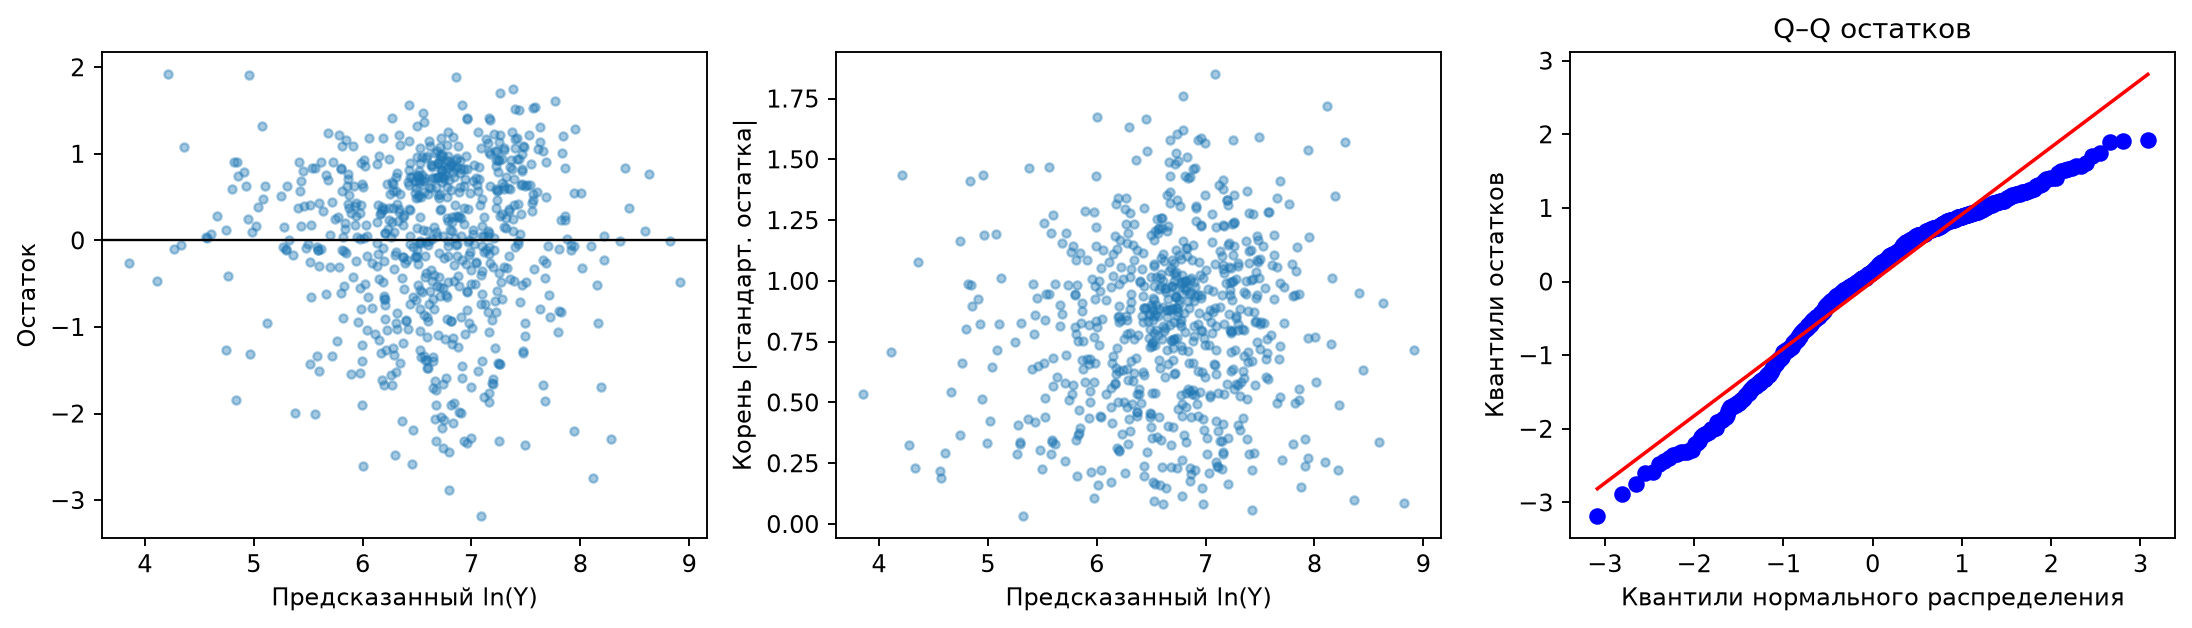
\includegraphics[width=0.98\textwidth,height=.38\textheight,keepaspectratio]{figures/diagnostics.png}
\caption{Остатки, их разброс и Q--Q-диаграмма M3}\label{learn:diagnostics}
\end{figure}

\textbf{Левая панель.} По горизонтали --- рассчитанный моделью логарифм суммы продаж, по вертикали --- остаток $e_i=y_i-\widehat y_i$. Каждая точка --- строка обучающей выборки. Горизонтальная линия отмечает ноль. Выше линии модель недооценила наблюдение, ниже --- переоценила. Большая положительная или отрицательная величина означает большое отклонение на логарифмической шкале.

Ищем форму, которую модель пропустила: например, явную дугу или систематический сдвиг остатка. Также смотрим, не расширяется ли облако при росте предсказания. У нас остатки есть с обеих сторон, отрицательный хвост длиннее. Сам факт расположения вокруг нуля не доказывает качество: у МНК с константой сумма обучающих остатков и так близка к нулю.

\textbf{Средняя панель.} По горизонтали то же предсказание. По вертикали --- $\sqrt{|e_i/s_e|}$, где $s_e$ --- выборочное стандартное отклонение остатков. Модуль убирает знак, корень сжимает большие значения. Панель помогает сравнить величину отклонений при разных уровнях предсказания. Это не стандартная ошибка коэффициента и не доверительный интервал. Неодинаковый разброс требует осторожности; без отдельной проверки по картинке нельзя объявить дисперсию постоянной.

\textbf{Правая панель: Q--Q.} По горизонтали --- теоретические квантили нормального распределения, по вертикали --- упорядоченные остатки. Если форма близка к нормальной, точки примерно лежат на опорной красной прямой. Она не является линией регрессии суммы продаж на фактор. У нас есть отклонения в хвостах и асимметрия; это не идеальная нормальная форма.

\textbf{Что нам это дало.} Получили диагностические признаки ограничений модели и основания осторожно обсуждать её точность. Дополнительно проверили один квадратичный член. Кластеризация была выбрана по повторным товарам; она не гарантирует устранения кривизны, смещения коэффициентов или общих шоков разных товаров.

\warning{Все три панели построены по остаткам на обучении. Они не заменяют проверку на исключённых товарах. Отсутствие заметного рисунка не доказывает, что выполнены все предпосылки.}

\answer{Эти графики отвечают на вопросы о форме и разбросе ошибок модели. У нас видна асимметрия остатков, поэтому я не называю модель идеальной. Качество вне обучения оценено отдельно.}


\section{Зачем 52 раза исключали товар}

Возможно, оценку определяет один необычный товар. Чтобы это проверить, удаляем все строки одного товара, оцениваем модель заново, возвращаем его и удаляем следующий. Получаем 52 набора коэффициентов.

Покупатели: диапазон 0,661--0,722, знак всегда положительный. Второй конкурент: 0,157--0,528, тоже положительный знак, но более заметный разброс величины. Рейтинг меняет знак в 10 случаях, доставка --- в 27.

Это показывает чувствительность оценок к отдельным товарам. Диапазон минимум--максимум не является 95\%-ным интервалом: процедура не калибрована на такое покрытие. Сохранение знака не означает сохранения значимости. И эта проверка не отвечает, что будет при одновременном удалении целой группы товаров.

\answer{Я проверил, не держится ли направление оценки на одном товаре. Покупатели устойчивы по знаку, рейтинг и доставка неустойчивы. На основании проверки товары из окончательной выборки не удалялись.}


\subsection{Почему понадобилось проверить время}

Исключение товара и добавление месяцев проверяют разные вещи. Первое спрашивает, не держится ли оценка на конкретном объекте. Второе --- не объясняется ли часть связи общими изменениями периода: например, продажи и конкурентные цены могли одновременно меняться в одном месяце.

К M3 добавили 19 индикаторов конкретных календарных месяцев. Всего месяцев 20, один базовый --- январь 2017. Это не только сезонность «январь против февраля»: январь 2017 и январь 2018 получают разные эффекты. Уравнение и исходная выборка остаются прежними по остальным признакам. Число коэффициентов возрастает с 18 до 37; кластеров по-прежнему 52. Поправка Холма в обеих моделях относится к тем же девяти числовым коэффициентам, а не ко всем временным индикаторам.


\begin{tabular}{lrrr}
\toprule
Спецификация & Параметров & $p$ конкурентов & $p_{Holm}$ веса \\
\midrule
M3 & 18 & 0,011 & 0,049 \\
M3 + месяцы & 37 & 0,061 & 0,116 \\
\bottomrule
\end{tabular}


\textbf{Как прочитать результат.} В основной M3 совместное p-value конкурентов 0,011, после календарного контроля --- 0,061. Раньше правило на уровне 5\% отвергало гипотезу о трёх нулевых коэффициентах, теперь не отвергает. Для веса после Холма 0,049 сменяется на 0,116. Оба статистических решения чувствительны к спецификации.

\textbf{Что из этого следует.} Правильно сказать: «В основной модели обнаружена совместная связь; при учёте времени её статистическое подтверждение ослабевает». Неправильно сказать: «Время доказало отсутствие связи» или «выбираем модель без месяцев, потому что там есть значимость». Коэффициенты конкурентов остаются положительными, но неопределённость и сами оценки меняются. Две разные значимости не заменяют специального теста различия коэффициентов.

\textbf{Почему M3 не удалили?} Это основная заранее заданная спецификация. Дополнительная модель появилась после замечания при проверке работы и честно представлена как анализ чувствительности. Она тоже не гарантирует правильность: много коэффициентов относительно 52 товарных групп, а возможная зависимость ошибок разных товаров остаётся. Оценка качества предсказания M1--M3 не пересчитывалась под новую цель; календарное расширение здесь не объявляется проверенной моделью будущего прогноза.

\answer{Я дополнительно учёл каждый календарный месяц. Совместное p-value конкурентов выросло с 0,011 до 0,061, а p-value веса после Холма --- с 0,049 до 0,116. Поэтому основной вывод нужно считать чувствительным к учёту времени, а не безусловно устойчивым.}

\section{Почему проверяем предсказание отдельно}

На обучении модель видела значения отклика и подстраивала коэффициенты под них. Проверка на тех же данных может скрывать переобучение: дополнительные столбцы помогают объяснить частные особенности исходной выборки, которые не повторяются у исключённых товаров.

Пять частей разделены по \texttt{product\_id}. В каждом шаге четыре части обучающие, пятая проверочная. Каждый товар один раз оказывается в проверке. Отдельные строки товара не разделяются между обучением и проверкой.

Обычный GroupKFold не обеспечил покрытие категорий в каждом обучении. Поэтому использован предусмотренный алгоритм распределения товаров внутри категорий, без значений отклика. Фиксирован seed 20261030 --- начальное состояние генератора, позволяющее воспроизвести разбиение. Число проверочных товаров: 11, 11, 10, 10, 10.

При каждом шаге коэффициенты оцениваются заново. Для ориентира используется средний логарифм отклика только обучающих строк. Все модели проверяются на одинаковых исключённых строках.

Категории известны, поскольку задача относится к новым товарам уже представленного ассортимента. Это не проверка неизвестной категории. В разных частях также присутствуют те же исторические месяцы, а покупатели и цены заданы как известные признаки. Это не проверка будущих месяцев и не готовая система прогнозирования заранее.

\section{RMSE и MAE: что означают числа около единицы}

\[
 RMSE=\sqrt{\frac1n\sum_i(y_i-\widehat y_i^{out})^2},\qquad
 MAE=\frac1n\sum_i|y_i-\widehat y_i^{out}|.
\]
$\widehat y_i^{out}$ --- предсказание для строки, товар которой отсутствовал в обучении. RMSE сильнее реагирует на крупные ошибки. MAE --- средняя абсолютная ошибка. Каждая строка имеет одинаковый вес; товары с большим числом месяцев дают больше строк.

\begin{center}\small\begin{tabular}{lrrrr}
\toprule
Модель & RMSE & MAE & $R^2$ & SD(RMSE) \\
\midrule
Mean & 1,199 & 0,982 & -0,009 & 0,077 \\
M1 & 1,043 & 0,853 & 0,238 & 0,079 \\
M2 & 1,030 & 0,833 & 0,256 & 0,072 \\
M3 & 1,033 & 0,836 & 0,252 & 0,100 \\
\bottomrule
\end{tabular}\end{center}

Ошибки выражены в единицах натурального логарифма. RMSE 1,033 не означает 1,033\% ошибки и не означает почти идеальное предсказание. Поскольку шкала логарифмическая, даже единица соответствует заметному мультипликативному отличию, но экспонента RMSE не является автоматически средней относительной ошибкой.

M2 и M3 лучше простого среднего на выбранном разбиении. M3 имеет ошибку немного выше M2: дополнительные факторы не дали выигрыша совокупной RMSE и MAE. Это согласуется с неподтверждённым совместным вкладом добавленного блока, но тест значимости и предсказательная ошибка всё же отвечают на разные вопросы.

Столбец SD(RMSE) показывает разброс пяти ошибок частей. Он не является стандартной ошибкой среднего независимых экспериментов: обучающие наборы пересекаются. Мы не строили по нему тест превосходства M2 над M3. Одно разбиение не гарантирует тот же порядок при других частях.


\subsection{Две панели предсказания: как увидеть качество вне обучения}

\begin{figure}[H]\centering
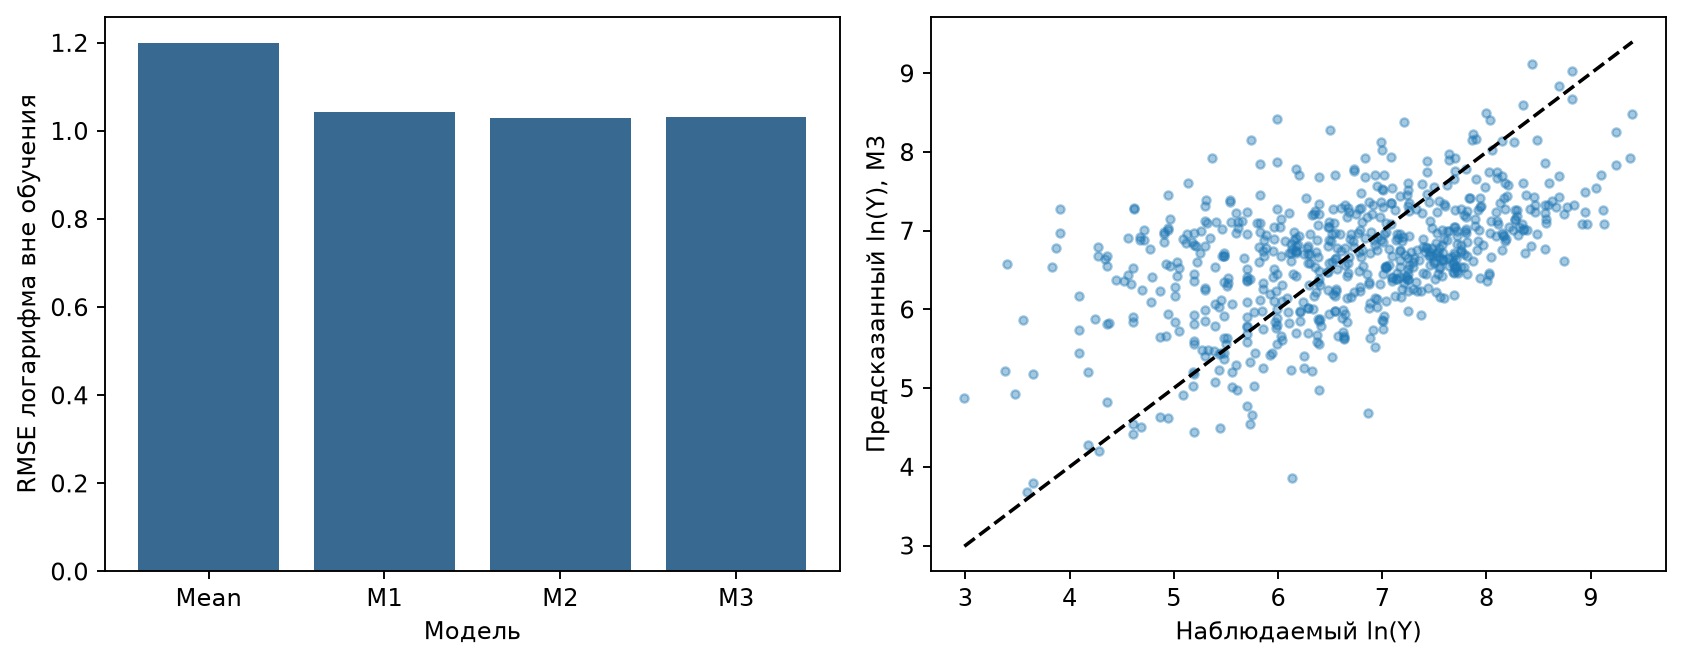
\includegraphics[width=0.98\textwidth,height=.43\textheight,keepaspectratio]{figures/validation.png}
\caption{Ошибка на исключённых товарах и их предсказания M3}\label{learn:validation}
\end{figure}

\textbf{Левая панель.} По горизонтали --- варианты модели; Mean означает простой прогноз среднего обучающего логарифма. По вертикали --- совокупная RMSE вне обучения, в единицах логарифма. Ниже столбец --- меньше ошибка. Это не доля правильно классифицированных товаров.

У нас среднее даёт 1,199, M1 --- 1,043, M2 --- 1,030, M3 --- 1,033. Различие M2 и M3 очень небольшое, поэтому столбцы визуально почти одинаковы. Главный вывод: новые признаки не снизили ошибку на этом разбиении. На столбцах нет доверительных интервалов, и формальная значимость разности не проверялась.

\textbf{Правая панель.} По горизонтали --- наблюдаемый логарифм суммы продаж, по вертикали --- предсказанный логарифм. Каждая точка --- строка, для которой модель обучалась без соответствующего товара. Пунктирная диагональ --- точное совпадение $\widehat y=y$.

Точка на диагонали означает точное предсказание логарифма. Выше диагонали предсказание слишком велико; ниже --- слишком мало. Это важно не перепутать с графиком остатков, где по вертикали было «наблюдаемое минус предсказанное». Чем дальше точки от диагонали, тем больше ошибки.

\textbf{Что видно у нас.} Общее положительное направление есть, но облако довольно широкое. Предсказания сжаты к средним уровням: крайние низкие значения часто переоцениваются, высокие --- недооцениваются. Поэтому даже преимущество над простым средним не означает точного предсказания каждой строки.

\textbf{Что нам это дало.} Проверили пользу модели на исключённых товарах, а не только на данных подгонки. Выявили различие задач: M3 подробнее описывает исходные связи, но M2 имеет немного меньшую совокупную ошибку.

\warning{Все точки на правой панели принадлежат одной M3; четыре столбца слева сравнивают разные варианты. Величины на обеих панелях логарифмические. Общие исторические месяцы и известные категории сохраняются: это не тест будущего периода.}

\answer{Слева сравниваются ошибки вне обучения: меньше --- лучше. Справа видно, насколько предсказания исключённых товаров близки к точным значениям. Дополнительные признаки не дали выигрыша на выбранном разбиении, а разброс ошибок остаётся заметным.}


\section{Почему выводы ограничены}

\begin{enumerate}
\item \textbf{Наблюдательные данные.} Продажи, конкуренция и активность покупателей могут зависеть от общих причин. Регрессия не заменяет эксперимент.
\item \textbf{52 товара.} Это небольшой набор для оценки различий свойств. В двух категориях только два товара.
\item \textbf{Общие шоки.} Кластеризация по товару допускает зависимость внутри товара, но не произвольную зависимость разных товаров. Особенно осторожен пограничный результат веса.
\item \textbf{Неполная документация.} Не установлен весь механизм построения агрегатов и сопоставления конкурентов.
\item \textbf{Нет индивидуальных эффектов товаров; время проверено дополнительно.} Категория не контролирует все постоянные свойства товара; в основной M3 возможны пропущенные календарные изменения; добавление месяцев показывает чувствительность вывода.
\item \textbf{Данные уже изучались.} Анализ поисковый; текущая проверка не является независимым подтверждением заранее зарегистрированной гипотезы.
\end{enumerate}

Ограничения не означают, что все расчёты бессмысленны. Они задают точную область утверждения: при таком наборе данных и такой модели получены такие оценки и свидетельства. Сильнее этого заявлять нельзя.

\section{Ответы на вероятные вопросы}

\subsection*{Что именно вы сделали самостоятельно?}
\answer{Проверил структуру и смысл данных, выбрал признаки, сравнил спецификации, рассчитал кластерные проверки и интервалы, выполнил диагностику и анализ чувствительности, организовал проверку на исключённых товарах и сопоставил результаты. Расчёты воспроизводятся одним исходником и ноутбуком.}

\subsection*{Почему это множественная регрессия?}
\answer{Отклик объясняется несколькими признаками одновременно. В полной модели девять числовых факторов и индикаторы категорий.}

\subsection*{Почему вы исследуете сумму продаж, если тема про розничную торговлю?}
\answer{Тема охватывает розничные данные в целом. Сумма продаж --- содержательный результат торговли. Я явно определил отклик и не подменяю его ценой единицы.}

\subsection*{Почему оставили все три цены, если отдельно они незначимы?}
\answer{Они составляют основной исследовательский блок. Отдельная незначимость после Холма не доказывает отсутствия совместной информации. Совместная гипотеза о трёх нулевых коэффициентах отвергается при принятой модели ошибок.}

\subsection*{Какой конкурент самый важный?}
\answer{По этим результатам уверенно ранжировать конкурентов нельзя. Различие p-value не является тестом различия коэффициентов. Основной вывод касается блока конкурентных цен и его чувствительности к календарному контролю.}

\subsection*{Зачем рейтинг и доставка, если от них нет значимости?}
\answer{Их включили по содержательному основанию. Сравнение показало, что совместный вклад трёх новых характеристик не подтверждён и ошибка не улучшилась. Это результат исследования, а не причина скрыть эти факторы.}

\subsection*{Почему не использовали все признаки или автоматический отбор?}
\answer{Среди столбцов есть идентификаторы, почти арифметические составляющие отклика и недостаточно описанные поля. Я выбрал фиксированные содержательные спецификации и показал их сравнение, чтобы не подбирать удачные p-value перебором.}

\subsection*{Почему не удалили первый конкурент с VIF больше пяти?}
\answer{Пять --- диагностический ориентир. Точного дублирования нет, а конкурент входит в основной вопрос. Я сохранил его и осторожно интерпретировал индивидуальные оценки.}

\subsection*{Что означает константа?}
\answer{Это базовый уровень линейного предсказания при нулевых значениях модельных числовых столбцов и базовой категории. Для логарифмированных столбцов ноль означает исходное значение один. Такое сочетание может быть вне реальных данных, поэтому я не придаю константе самостоятельного коммерческого смысла.}

\subsection*{Значимость --- это сильный эффект?}
\answer{Нет. Значимость учитывает оценку относительно её неопределённости, а величину связи показывает коэффициент и процентная интерпретация. Для практической оценки важен также интервал.}

\subsection*{При p больше 0,05 связи нет?}
\answer{Нет, данных недостаточно, чтобы отвергнуть нулевую гипотезу в данной модели. Возможны слабая связь, высокая неопределённость, небольшой диапазон фактора или недостаток независимых товаров.}

\subsection*{Почему 95\%-ный интервал не равен плюс-минус 1,96 ошибки?}
\answer{Здесь используется t-приближение с 51 степенью свободы; квантиль около 2,008. Число 1,96 относится к стандартному нормальному распределению.}

\subsection*{Что лучше: M2 или M3?}
\answer{M3 подробнее исследует условные связи и лучше подгоняет исходные данные. У M2 немного меньше ошибка на выбранных исключённых товарах. Я не заявляю статистически доказанного превосходства и не смешиваю эти две цели.}

\subsection*{Можно ли прогнозировать следующий месяц?}
\answer{Такую задачу мы не проверяли. Будущие покупатели и конкурентные цены заранее неизвестны; разбиение было по товарам, а не по времени. Для будущего прогноза нужны временная проверка и доступные на момент прогноза признаки.}

\subsection*{Какая предпосылка остаётся самой уязвимой?}
\answer{Независимость ошибок разных товаров: возможны общие шоки категории и месяца. Также неполное описание агрегатов. Я указал, что p-value условны на принятой схеме ошибок.}

\subsection*{Что можно улучшить дальше?}
\answer{Уточнить происхождение данных, расширить число товаров и период, углубить анализ временных изменений, добавить индивидуальные эффекты и проверить более общую зависимость ошибок. Календарная чувствительность уже оценена и показала ослабление основного вывода. Это потребует отдельного этапа, особенно потому, что категории немногочисленны.}

\section{Как читать каждый слайд}

\begin{longtable}{p{.06\textwidth}p{.38\textwidth}p{.47\textwidth}}
\toprule № & Что показываем & Что слушатель должен понять\\\midrule\endhead
1 & Тема и автор & Изучаем связи суммы продаж с несколькими факторами.\\
2 & Данные и распределение & Строка --- товар--месяц; отклик --- сумма, логарифм выбран осмысленно.\\
3 & Подготовка и признаки & Сохранение строк обосновано; набор факторов выбран по содержанию.\\
4 & M1--M3 и методы & Есть последовательное расширение, единая выборка и корректное различие подгонки/предсказания.\\
5 & Таблица коэффициентов и проверки & Конкуренты значимы совместно; отдельный не выделяется после Холма. Интервалы индивидуальные.\\
6 & Устойчивость к товарам и времени & Линия --- диапазон исключений, не доверительный интервал. Календарный контроль меняет p-value конкурентов с 0,011 до 0,061.\\
7 & Проверка качества & Целые товары исключаются из обучения; добавление признаков не дало выигрыша ошибки.\\
8 & Выводы и ограничения & Совместная связь в основной модели чувствительна к календарному контролю; расширение признаков не улучшило предсказание.\\
9--10 & Резерв & Уточнение статистических проверок, диагностики и ограничений по вопросу комиссии.\\
\bottomrule\end{longtable}

\section{Ошибки, которых стоит избегать в устном ответе}

\begin{itemize}
\item Не заменяйте «сумма продаж» словом «цена», когда речь об отклике.
\item Не называйте 676 строк 676 независимыми товарами.
\item Не говорите, что M3 лучше во всех смыслах: вне обучения она не улучшила ошибку.
\item Не говорите, что третий конкурент доказанно важен после поправки.
\item Не путайте индивидуальные интервалы с одновременными для всех коэффициентов.
\item Не называйте p-value вероятностью истинности гипотезы.
\item Не говорите, что p=0,202 доказывает отсутствие всех нелинейностей.
\item Не называйте сохранение знака сохранением значимости.
\item Не интерпретируйте RMSE логарифма как процент ошибки.
\item Не превращайте условные связи в советы менять вес товара, число фото или цены.
\end{itemize}

На слайде 7 ошибки показаны горизонтальными столбцами: короче столбец --- меньше RMSE. Это те же численные результаты, что и на учебном рисунке проверки, но в более простом формате. Диагностические остатки перенесены на резервный слайд 10.

Если забыли конкретную цифру, сначала объясните проверяемый вопрос и смысл результата, затем посмотрите на таблицу. Не нужно заменять непонимание формул перечислением библиотек. Убедительный ответ связывает метод с вопросом и ограничивает вывод тем, что действительно проверено.

\section{Где в проекте найти подтверждение}

\begin{itemize}
\item \texttt{analysis\_retail.py}: общий исходник вычислений.
\item \texttt{science\_work\_simple.ipynb}: выполненные ячейки с таблицами и рисунками.
\item \texttt{results/main\_coefficients.csv}: коэффициенты и Холм.
\item \texttt{results/joint\_tests.csv}: совместные тесты и кривизна.
\item \texttt{results/cv\_metrics.csv}: качество вне обучения.
\item \texttt{results/sensitivity.csv}: диапазоны исключения товара.
\item \texttt{results/column\_audit.csv}: аудит всех исходных полей.
\item \texttt{validate\_statistics.py}: независимая численная проверка; \texttt{REVIEW.md}: разбор ограничений.
\end{itemize}

Технические детали используемых функций: \href{https://www.statsmodels.org/stable/generated/statsmodels.regression.linear_model.RegressionResults.get_robustcov_results.html}{кластерные ошибки statsmodels}, \href{https://www.statsmodels.org/stable/generated/statsmodels.stats.multitest.multipletests.html}{поправки на множественные проверки}, \href{https://scikit-learn.org/stable/modules/generated/sklearn.model_selection.GroupKFold.html}{разделение по группам}. Объяснения в этом файле привязаны к нашей спецификации, а не ко всем возможным случаям применения методов.

\end{document}
